\documentclass[11pt,a4paper]{article}
\usepackage[margin=2.2cm]{geometry}
\usepackage[T1]{fontenc}
\usepackage{lmodern}
\usepackage{booktabs}
\usepackage{graphicx}
\usepackage{amsmath}
\usepackage{enumitem}
\usepackage{float}
\usepackage{xcolor}
\usepackage[hidelinks]{hyperref}
\usepackage{titlesec}

\titlespacing*{\section}{0pt}{6pt}{3pt}
\setlist{noitemsep,topsep=2pt,leftmargin=*}
\setlength{\parskip}{2pt}
\setlength{\abovecaptionskip}{3pt}
\setlength{\textfloatsep}{8pt}
% Placeholder marker for the ablation numbers (remove once filled in).
\newcommand{\TBD}[1]{\textcolor{red}{#1}}

\title{\vspace{-0.8cm}\textbf{Skin Lesion Image Segmentation}\\ \large Final Technical Summary}
\author{Ilmira Usmanova, Ilia Kulichenko, Alsu Nizamieva, Amira Nabiullina, Andrei Silantev\\
{\small\texttt{\{i.usmanova, i.kulichenko, a.nizamieva, a.nabiullina, a.silantev\}@innopolis.university}}}
\date{\vspace{-0.4cm}10 November 2026}

\begin{document}
\emergencystretch=1em
\maketitle
\vspace{-0.6cm}

\section{Problem and Question}

We segment skin lesions in dermoscopic images (binary mask: lesion vs.\ skin). \textbf{Question:} with the same
pretrained encoder and the same training pipeline, does replacing the \textbf{U-Net} decoder by the
\textbf{DeepLabV3+} decoder (atrous spatial pyramid pooling, larger receptive field) improve accuracy, and at what
computational cost?

\section{Dataset}

\textbf{ISIC 2018 Challenge, Task 1}: 2,594 official training dermoscopic images with expert binary masks
(206 different resolutions, from 576$\times$540 to 6748$\times$4499 px; the lesion covers 0.3--98.7\% of the
image, median 14\%). Every file was checked against the official archive checksums.
\textbf{Split:} ISIC contains repeated photographs of the same lesion, so a random split would leak copies into
validation. We split by \emph{groups}: images sharing a \texttt{patient\_id} or \texttt{lesion\_id} (ISIC metadata)
or detected as near-duplicates (SIFT matching + RANSAC check on all 3.36\,M image pairs, $\geq$8 inliers) always stay
together: \textbf{2,205 train / 389 validation} images (85/15, seed 42). The official 1,000-image test set was not used.
\textbf{Preprocessing:} resize to 256$\times$256 (area interpolation; masks nearest-neighbour), ImageNet normalisation.
Training augmentations: flips, 90$^\circ$ rotations, affine (scale 0.9--1.1, shift, $\pm30^\circ$), colour jitter.

\section{Method and Experimental Setup}

\textbf{Baseline:} U-Net; \textbf{second condition:} DeepLabV3+ (output stride 16, prediction at 1/4 resolution,
one skip connection). Both use the same \textbf{ImageNet-pretrained ResNet-34} encoder
(\texttt{segmentation\_models\_pytorch} 0.5.0), so only the decoder differs (24.4\,M vs.\ 22.4\,M parameters).
Identical training: BCE + Dice loss, AdamW (lr $10^{-4}$), batch 16, up to 50 epochs, early stopping on validation
Dice (patience 10). Each model was trained with \textbf{three seeds} (42, 1, 2) to separate the architecture effect
from run-to-run noise. \textbf{Metrics} (per image at threshold 0.5, then averaged): Dice, IoU, the ISIC thresholded
Jaccard (IoU $<0.65$ counts as 0), and HD95 boundary distance in pixels; plus training and inference time.
\textbf{Ablation / sensitivity:} (i) the binarisation threshold (0.1--0.9) on the trained checkpoints
(U-Net seed 42, DeepLabV3+ seeds 1, 2); (ii) the loss: BCE only and Dice only vs.\ BCE + Dice for U-Net, seed 42,
everything else fixed.

\section{Results}

\begin{table}[H]
\centering
\small
\begin{tabular}{lcc}
\toprule
\textbf{Validation, 389 images} (mean $\pm$ std over 3 seeds) & \textbf{U-Net} & \textbf{DeepLabV3+} \\
\midrule
Dice                                  & \textbf{0.903 $\pm$ 0.002} & 0.901 $\pm$ 0.002 \\
IoU                                   & \textbf{0.837 $\pm$ 0.003} & 0.834 $\pm$ 0.003 \\
ISIC thresholded Jaccard              & \textbf{0.797 $\pm$ 0.002} & 0.793 $\pm$ 0.005 \\
Failed images (IoU $<0.65$)           & \textbf{32.3 $\pm$ 0.6}    & 33.3 $\pm$ 2.1 \\
HD95 median / 95th percentile (px)    & 7.14 / 47.5                & \textbf{6.87 / 43.1} \\
Dice, lesions $<5\%$ of image ($n=90$) & \textbf{0.883 $\pm$ 0.007} & 0.875 $\pm$ 0.010 \\
\midrule
Inference per image (batch 1, MacBook Air M3, MPS) & \textbf{10.5\,ms} & 17.0\,ms \\
Training time per epoch, same machine & \textbf{70\,s} & 94\,s \\
Total training time (early stopping)  & 53.6 $\pm$ 12.4\,min & \textbf{47.7 $\pm$ 2.3\,min} \\
\bottomrule
\end{tabular}

\vspace{4pt}
\begin{tabular}{lccccc}
\toprule
\textbf{Loss ablation} (U-Net, seed 42) & \textbf{Dice} & \textbf{IoU} & \textbf{ISIC Jaccard} & \textbf{Failed} & \textbf{HD95 p95} \\
\midrule
BCE + Dice (baseline)      & \textbf{0.901} & \textbf{0.834} & \textbf{0.796} & \textbf{32} & 52.4 \\
BCE only                   & 0.897 & 0.828 & 0.778 & 41 & \textbf{52.0} \\
Dice only                  & 0.894 & 0.825 & 0.787 & 35 & 60.8 \\
\bottomrule
\end{tabular}
\caption{Main comparison (top) and loss ablation (bottom); bold = better value. Per-seed numbers:
\texttt{results/comparison/seeds\_summary.md}; ablation: \texttt{results/ablation/}.}
\label{tab:results}
\end{table}

\section{Interpretation}

The two decoders segment practically equally well: U-Net is ahead by 0.0024 Dice on average and in each of the three
seeds, but this gap is about the size of the run-to-run spread (std 0.002) and the 95\% bootstrap interval of the
per-image difference ($-0.006$ to $+0.001$) contains zero. The stable differences are small and follow from the
architecture: DeepLabV3+ is worse on small lesions ($-0.008$ Dice for lesions under 5\% of the image), because it
predicts the mask at 1/4 resolution with only one skip connection, while its wider context gives fewer extreme border errors (HD95 95th percentile 43 vs.\ 48\,px). DeepLabV3+ is also 1.3$\times$ slower to train per epoch and
1.6$\times$ slower at inference (its dilated last stage works on 16$\times$16 maps).
\textbf{Threshold:} 0.5 is near-optimal for both models (the best, 0.4, gains $\leq$0.0004 Dice; over 0.3--0.7
Dice changes by $\leq$0.006), so the comparison does not depend on it; only 0.1 or 0.9 hurt ($-0.012$ to $-0.031$).
\textbf{Loss:} BCE + Dice is best on every overlap metric; dropping a term costs 0.004 (BCE only) or 0.007
(Dice only) Dice, but with one seed and bootstrap intervals that include zero this is a trend, not a significant
effect. BCE only gives soft, poorly calibrated probabilities (Dice spread 0.027 over thresholds 0.3--0.7) and
under-segments at 0.5 (9 more failures); Dice only gives near-binary outputs but stops early (best epoch 10) and
has the worst boundary outliers (HD95 p95 60.8 vs.\ 52.4\,px), because without the per-pixel BCE term isolated
wrong regions are penalised less.

\section{Failure Analysis}

\begin{figure}[H]
\centering
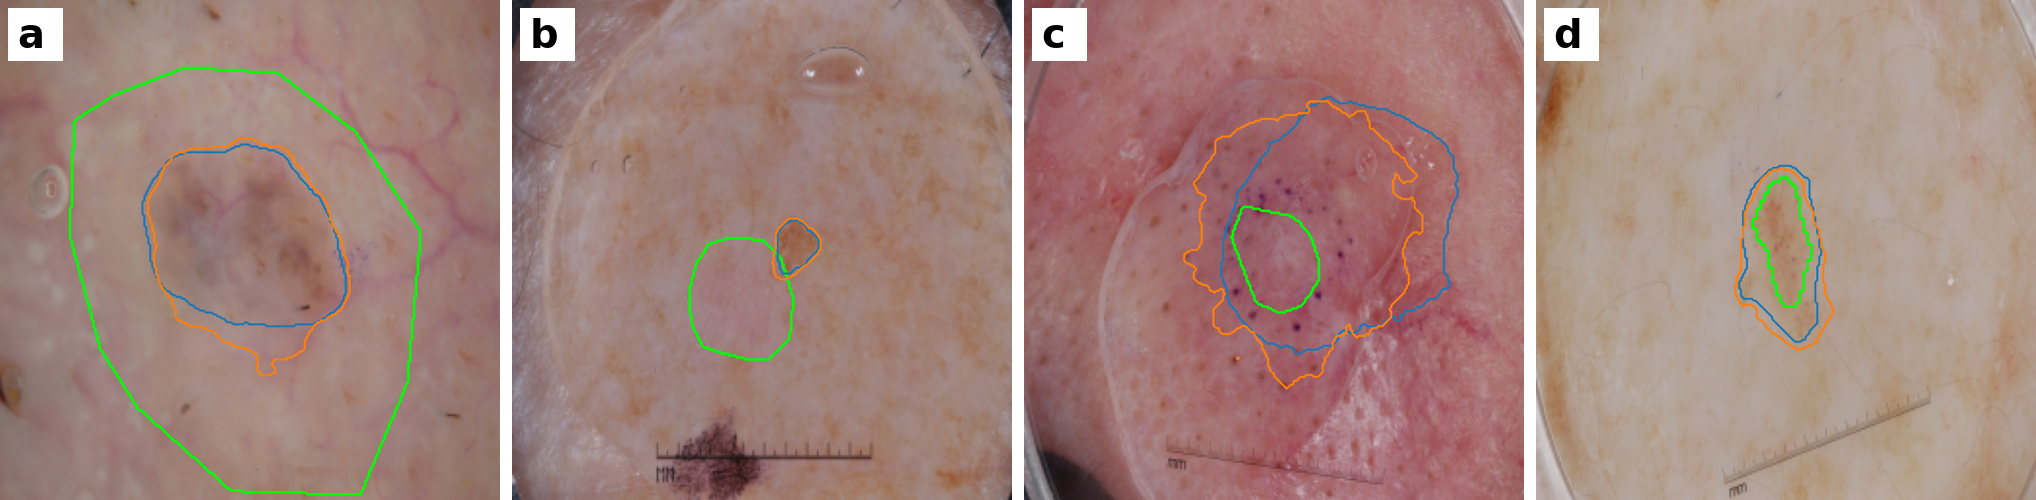
\includegraphics[width=\linewidth]{figures/failure_row.png}
\caption{Failures shared by all six runs (IoU $<0.65$ in every seed of both models). Green = ground truth,
blue = U-Net, orange = DeepLabV3+.}
\label{fig:failures}
\end{figure}

13 images fail (IoU $<0.65$) in all six runs, so these failures are properties of the image, not of one run.
\textbf{(a) Annotation ambiguity} (Dice 0.38--0.44): the ground truth is a coarse polygon that includes a wide,
barely coloured halo, while both models outline the visible pigmented centre.
\textbf{(b) Wrong object} (Dice $\leq$0.04 in 5 of 6 runs): the annotated lesion is a faint pink, almost unpigmented
melanoma; both models segment a nearby brown spot with higher contrast, because training data are dominated by
brown, well-pigmented lesions.
\textbf{(c) Artefact edge} (Dice 0.13--0.33): a fold of immersion fluid under the contact plate forms the strongest
closed contour around a light lesion, and the models follow it.
\textbf{(d) Small lesion with a diffuse border} (Dice 0.61--0.67 U-Net, 0.53--0.58 DeepLabV3+): both models
over-segment, DeepLabV3+ more so in every seed, which matches its coarser output. Cases (b) and (c) also explain why the better boundary statistics of DeepLabV3+ do not reduce the number
of failures: its wider context shortens border errors but does not help when the wrong region is chosen.

\section{Conclusions and Limitations}

With a shared pretrained encoder and pipeline, the decoder choice has almost no effect on overall accuracy
(Dice $\approx$0.90 for both); the remaining errors come mostly from the data (annotation style, weakly pigmented
lesions, contact-plate artefacts) and are shared by both models. The ablation supports the combined
BCE + Dice loss and the default threshold 0.5 are sound choices. In our setting the simpler and faster
\textbf{U-Net is the better choice}. \textbf{Limitations:} (i) all numbers are on our 389-image validation split,
which was also used for early stopping, so they may be slightly optimistic; the official test set was not evaluated;
(ii) three seeds, one split and one image size (256$\times$256, which removes fine border detail);
(iii) failure causes are read from the images, not tested by targeted experiments; (iv) timings come from fanless
laptops that throttle (10--20\% variation).

\section{Reproducibility}

\textbf{Code:} \url{https://github.com/amiranabiullina/skin_lesions_CV_project} (README with setup, data download, training, evaluation and ablation commands; committed split, configs,
per-image metrics, logs and figures).
\textbf{Environment:} Python 3.14, PyTorch 2.14.1 (MPS), segmentation\_models\_pytorch 0.5.0, Albumentations 2.0.8;
pinned \texttt{requirements.txt}. Trained on Apple-silicon MacBook Air laptops (M3/M4, MPS): about 50\,min per run; inference 10--17\,ms per image.

\section{Members' Contributions}
\begin{center}
\small
\begin{tabular}{@{}ll@{}}
\toprule
\textbf{Member} & \textbf{Contribution} \\
\midrule
Ilmira Usmanova  & Evaluation script (Dice, IoU, HD95), result tables and figures \\
Ilia Kulichenko  & Training script and U-Net baseline experiments \\
Alsu Nizamieva   & DeepLabV3+ experiments and runtime measurements \\
Amira Nabiullina & Dataset code, preprocessing and splits; ablation; coordination, README and summary \\
Andrei Silantev  & Boundary and failure-case analysis \\
\bottomrule
\end{tabular}
\end{center}

\end{document}
